\documentclass[../psets.tex]{subfiles}

\pagestyle{main}
\renewcommand{\leftmark}{Problem Set 2}

\begin{document}




\begin{enumerate}[label={\Roman*)}]
    \item \marginnote{1/28:}Do the following problem from your text: Chapter 4: \#22.
    \begin{enumerate}[label={\textbf{4.\arabic*}}]
        \setcounter{enumii}{21}
        \item Using the $D_{2d}$ character table,
        \begin{enumerate}[label={\textbf{\alph*.}}]
            \item Determine the order of the group.
            \begin{proof}[Answer]
                $h=8$; count the number of symmetry elements.
            \end{proof}
            \item Verify that the $E$ irreducible representation is orthogonal to each of the other irreducible representations.
            \begin{proof}[Answer]
                \begin{align*}
                    \sum_{R_c}g_c\chi_E(R_c)\chi_{A_1}(R_c) &= (1)(2)(1)+(2)(0)(1)+(1)(-2)(1)+(2)(0)(1)+(2)(0)(1) = 0\\
                    \sum_{R_c}g_c\chi_E(R_c)\chi_{A_2}(R_c) &= (1)(2)(1)+(2)(0)(1)+(1)(-2)(1)+(2)(0)(-1)+(2)(0)(-1) = 0\\
                    \sum_{R_c}g_c\chi_E(R_c)\chi_{B_1}(R_c) &= (1)(2)(1)+(2)(0)(-1)+(1)(-2)(1)+(2)(0)(1)+(2)(0)(-1) = 0\\
                    \sum_{R_c}g_c\chi_E(R_c)\chi_{B_2}(R_c) &= (1)(2)(1)+(2)(0)(-1)+(1)(-2)(1)+(2)(0)(-1)+(2)(0)(1) = 0
                \end{align*}
            \end{proof}
            \item For each of the irreducible representations, verify that the sum of the squares of the characters equals the order of the group.
            \begin{proof}[Answer]
                \begin{align*}
                    \sum_{R_c}g_c[\chi_{A_1}(R_c)]^2 &= 1\cdot 1^2+2\cdot 1^2+1\cdot 1^2+2\cdot 1^2+2\cdot 1^2 = 8\\
                    \sum_{R_c}g_c[\chi_{A_2}(R_c)]^2 &= 1\cdot 1^2+2\cdot 1^2+1\cdot 1^2+2\cdot (-1)^2+2\cdot (-1)^2 = 8\\
                    \sum_{R_c}g_c[\chi_{B_1}(R_c)]^2 &= 1\cdot 1^2+2\cdot (-1)^2+1\cdot 1^2+2\cdot 1^2+2\cdot (-1)^2 = 8\\
                    \sum_{R_c}g_c[\chi_{B_2}(R_c)]^2 &= 1\cdot 1^2+2\cdot (-1)^2+1\cdot 1^2+2\cdot (-1)^2+2\cdot 1^2 = 8\\
                    \sum_{R_c}g_c[\chi_{E}(R_c)]^2   &= 1\cdot 2^2+2\cdot 0^2+1\cdot (-2)^2+2\cdot 0^2+2\cdot 0^2 = 8
                \end{align*}
            \end{proof}
            \item Reduce the following representations to their component irreducible representations.
            \begin{center}
                \vspace{1em}
                \small
                \renewcommand{\arraystretch}{1.2}
                \begin{tabular}{l|ccccc}
                    \noalign{\global\arrayrulewidth=0.5pt}\arrayrulecolor{grx}\hline
                    \rowcolor{gax}
                    $D_{2d}$ & $E$ & $2S_4$ & $C_2$ & $2C_2'$ & $2\sigma_d$\\
                    \hline
                    $\Gamma_1$ & 6 & 0 & 2 & 2 & 2\\
                    $\Gamma_2$ & 6 & 4 & 6 & 2 & 0\\
                    \hline
                \end{tabular}
                \vspace{1em}
            \end{center}
            \begin{proof}[Answer]
                For $\Gamma_1$:
                \begingroup
                \allowdisplaybreaks
                \begin{align*}
                    \hspace{-4em}a_{A_1} &= \frac{1}{8}\sum_{R_c}g_c\chi_{\Gamma_1}(R_c)\chi_{A_1}(R_c) = \frac{1}{8}[(1)(6)(1)+(2)(0)(1)+(1)(2)(1)+(2)(2)(1)+(2)(2)(1)] = 2\\
                    \hspace{-4em}a_{A_2} &= \frac{1}{8}\sum_{R_c}g_c\chi_{\Gamma_1}(R_c)\chi_{A_2}(R_c) = \frac{1}{8}[(1)(6)(1)+(2)(0)(1)+(1)(2)(1)+(2)(2)(-1)+(2)(2)(-1)] = 0\\
                    \hspace{-4em}a_{B_1} &= \frac{1}{8}\sum_{R_c}g_c\chi_{\Gamma_1}(R_c)\chi_{B_1}(R_c) = \frac{1}{8}[(1)(6)(1)+(2)(0)(-1)+(1)(2)(1)+(2)(2)(1)+(2)(2)(-1)] = 1\\
                    \hspace{-4em}a_{B_2} &= \frac{1}{8}\sum_{R_c}g_c\chi_{\Gamma_1}(R_c)\chi_{B_2}(R_c) = \frac{1}{8}[(1)(6)(1)+(2)(0)(-1)+(1)(2)(1)+(2)(2)(-1)+(2)(2)(1)] = 1\\
                    \hspace{-4em}a_{E}   &= \frac{1}{8}\sum_{R_c}g_c\chi_{\Gamma_1}(R_c)\chi_{E}(R_c)   = \frac{1}{8}[(1)(6)(2)+(2)(0)(0)+(1)(2)(-2)+(2)(2)(0)+(2)(2)(0)] = 1
                \end{align*}
                \endgroup
                Therefore, we know that
                \begin{equation*}
                    \Gamma_1 = 2A_1+B_1+B_2+E
                \end{equation*}
                For $\Gamma_2$:
                \begin{align*}
                    \hspace{-4em}a_{A_1} &= \frac{1}{8}\sum_{R_c}g_c\chi_{\Gamma_2}(R_c)\chi_{A_1}(R_c) = \frac{1}{8}[(1)(6)(1)+(2)(4)(1)+(1)(6)(1)+(2)(2)(1)+(2)(0)(1)] = 3\\
                    \hspace{-4em}a_{A_2} &= \frac{1}{8}\sum_{R_c}g_c\chi_{\Gamma_2}(R_c)\chi_{A_2}(R_c) = \frac{1}{8}[(1)(6)(1)+(2)(4)(1)+(1)(6)(1)+(2)(2)(-1)+(2)(0)(-1)] = 2\\
                    \hspace{-4em}a_{B_1} &= \frac{1}{8}\sum_{R_c}g_c\chi_{\Gamma_2}(R_c)\chi_{B_1}(R_c) = \frac{1}{8}[(1)(6)(1)+(2)(4)(-1)+(1)(6)(1)+(2)(2)(1)+(2)(0)(-1)] = 1\\
                    \hspace{-4em}a_{B_2} &= \frac{1}{8}\sum_{R_c}g_c\chi_{\Gamma_2}(R_c)\chi_{B_2}(R_c) = \frac{1}{8}[(1)(6)(1)+(2)(4)(-1)+(1)(6)(1)+(2)(2)(-1)+(2)(0)(1)] = 0\\
                    \hspace{-4em}a_{E}   &= \frac{1}{8}\sum_{R_c}g_c\chi_{\Gamma_2}(R_c)\chi_{E}(R_c)   = \frac{1}{8}[(1)(6)(2)+(2)(4)(0)+(1)(6)(-2)+(2)(2)(0)+(2)(0)(0)] = 0
                \end{align*}
                Therefore, we know that
                \begin{equation*}
                    \Gamma_2 = 3A_1+2A_2+B_1
                \end{equation*}
            \end{proof}
        \end{enumerate}
    \end{enumerate}
    \newpage
    \item Decompose the following reducible representations into their irreducible components. Ordering of the classes is the same as in the character tables in Appendix C of your text.
    \begin{enumerate}[label={\alph*)}]
        \item $D_{3h}$: $5,2,1,3,0,3$
        \begin{proof}[Answer]
            \begin{align*}
                \hspace{-4em}a_{A_1'}  &= \frac{1}{12}\sum_{R_c}g_c\chi_\Gamma(R_c)\chi_{A_1'}(R_c)  = \frac{1}{12}[(1)(5)(1)+(2)(2)(1)+(3)(1)(1)+(1)(3)(1)+(2)(0)(1)+(3)(3)(1)] = 2\\
                \hspace{-4em}a_{A_2'}  &= \frac{1}{12}\sum_{R_c}g_c\chi_\Gamma(R_c)\chi_{A_2'}(R_c)  = \frac{1}{12}[(1)(5)(1)+(2)(2)(1)+(3)(1)(-1)+(1)(3)(1)+(2)(0)(1)+(3)(3)(-1)] = 0\\
                \hspace{-4em}a_{E'}    &= \frac{1}{12}\sum_{R_c}g_c\chi_\Gamma(R_c)\chi_{E'}(R_c)    = \frac{1}{12}[(1)(5)(2)+(2)(2)(-1)+(3)(1)(0)+(1)(3)(2)+(2)(0)(-1)+(3)(3)(0)] = 1\\
                \hspace{-4em}a_{A_1''} &= \frac{1}{12}\sum_{R_c}g_c\chi_\Gamma(R_c)\chi_{A_1''}(R_c) = \frac{1}{12}[(1)(5)(1)+(2)(2)(1)+(3)(1)(1)+(1)(3)(-1)+(2)(0)(-1)+(3)(3)(-1)] = 0\\
                \hspace{-4em}a_{A_2''} &= \frac{1}{12}\sum_{R_c}g_c\chi_\Gamma(R_c)\chi_{A_2''}(R_c) = \frac{1}{12}[(1)(5)(1)+(2)(2)(1)+(3)(1)(-1)+(1)(3)(-1)+(2)(0)(-1)+(3)(3)(1)] = 1\\
                \hspace{-4em}a_{E''}   &= \frac{1}{12}\sum_{R_c}g_c\chi_\Gamma(R_c)\chi_{E''}(R_c)   = \frac{1}{12}[(1)(5)(2)+(2)(2)(-1)+(3)(1)(0)+(1)(3)(-2)+(2)(0)(1)+(3)(3)(0)] = 0
            \end{align*}
            Therefore, we know that
            \begin{equation*}
                \Gamma = 2A_1'+E'+A_2''
            \end{equation*}
        \end{proof}
        \item $D_{3h}$: $3,0,-1,-3,0,1$
        \begin{proof}[Answer]
            \begin{align*}
                \hspace{-4em}a_{A_1'}  &= \frac{1}{12}\sum_{R_c}g_c\chi_\Gamma(R_c)\chi_{A_1'}(R_c)  = \frac{1}{12}[(1)(3)(1)+(2)(0)(1)+(3)(-1)(1)+(1)(-3)(1)+(2)(0)(1)+(3)(1)(1)] = 0\\
                \hspace{-4em}a_{A_2'}  &= \frac{1}{12}\sum_{R_c}g_c\chi_\Gamma(R_c)\chi_{A_2'}(R_c)  = \frac{1}{12}[(1)(3)(1)+(2)(0)(1)+(3)(-1)(-1)+(1)(-3)(1)+(2)(0)(1)+(3)(1)(-1)] = 0\\
                \hspace{-4em}a_{E'}    &= \frac{1}{12}\sum_{R_c}g_c\chi_\Gamma(R_c)\chi_{E'}(R_c)    = \frac{1}{12}[(1)(3)(2)+(2)(0)(-1)+(3)(-1)(0)+(1)(-3)(2)+(2)(0)(-1)+(3)(1)(0)] = 0\\
                \hspace{-4em}a_{A_1''} &= \frac{1}{12}\sum_{R_c}g_c\chi_\Gamma(R_c)\chi_{A_1''}(R_c) = \frac{1}{12}[(1)(3)(1)+(2)(0)(1)+(3)(-1)(1)+(1)(-3)(-1)+(2)(0)(-1)+(3)(1)(-1)] = 0\\
                \hspace{-4em}a_{A_2''} &= \frac{1}{12}\sum_{R_c}g_c\chi_\Gamma(R_c)\chi_{A_2''}(R_c) = \frac{1}{12}[(1)(3)(1)+(2)(0)(1)+(3)(-1)(-1)+(1)(-3)(-1)+(2)(0)(-1)+(3)(1)(1)] = 1\\
                \hspace{-4em}a_{E''}   &= \frac{1}{12}\sum_{R_c}g_c\chi_\Gamma(R_c)\chi_{E''}(R_c)   = \frac{1}{12}[(1)(3)(2)+(2)(0)(-1)+(3)(-1)(0)+(1)(-3)(-2)+(2)(0)(1)+(3)(1)(0)] = 1
            \end{align*}
            Therefore, we know that
            \begin{equation*}
                \Gamma = A_2''+E''
            \end{equation*}
        \end{proof}
        \item $C_{2v}$: $4,0,0,0$
        \begin{proof}[Answer]
            We know the following by inspection.
            \begin{equation*}
                \Gamma = A_1+A_2+B_1+B_2
            \end{equation*}
        \end{proof}
        \item $C_{2h}$: $5,1,1,1$
        \begin{proof}[Answer]
            We know the following by inspection.
            \begin{equation*}
                \Gamma = 2A_g+B_g+A_u+B_u
            \end{equation*}
        \end{proof}
        \item $T_d$: $13,1,5,-3,-3$
        \begin{proof}[Answer]
            \begin{align*}
                \hspace{-3em}a_{A_1} &= \frac{1}{24}\sum_{R_c}g_c\chi_\Gamma(R_c)\chi_{A_1}(R_c) = \frac{1}{24}[(1)(13)(1)+(8)(1)(1)+(3)(5)(1)+(6)(-3)(1)+(6)(-3)(1)] = 0\\
                \hspace{-3em}a_{A_2} &= \frac{1}{24}\sum_{R_c}g_c\chi_\Gamma(R_c)\chi_{A_2}(R_c) = \frac{1}{24}[(1)(13)(1)+(8)(1)(1)+(3)(5)(1)+(6)(-3)(-1)+(6)(-3)(-1)] = 3\\
                \hspace{-3em}a_{E}   &= \frac{1}{24}\sum_{R_c}g_c\chi_\Gamma(R_c)\chi_{E}(R_c)   = \frac{1}{24}[(1)(13)(2)+(8)(1)(-1)+(3)(5)(2)+(6)(-3)(0)+(6)(-3)(0)] = 2\\
                \hspace{-3em}a_{T_1} &= \frac{1}{24}\sum_{R_c}g_c\chi_\Gamma(R_c)\chi_{T_1}(R_c) = \frac{1}{24}[(1)(13)(3)+(8)(1)(0)+(3)(5)(-1)+(6)(-3)(1)+(6)(-3)(-1)] = 1\\
                \hspace{-3em}a_{T_2} &= \frac{1}{24}\sum_{R_c}g_c\chi_\Gamma(R_c)\chi_{T_2}(R_c) = \frac{1}{24}[(1)(13)(3)+(8)(1)(0)+(3)(5)(-1)+(6)(-3)(-1)+(6)(-3)(1)] = 1
            \end{align*}
            Therefore, we know that
            \begin{equation*}
                \Gamma = 3A_2+2E+T_1+T_2
            \end{equation*}
        \end{proof}
        \item $T_h$: $8,-1,-1,4,8,-1,-1,4$
        \begin{proof}[Answer]
            With respect to the two doubly degenerate groups, we must add the two parts together and also double the order that we are dividing out. Note that $\varepsilon=\e[2\pi i/3]=\cos(\frac{2\pi}{3})+i\sin(\frac{2\pi}{3})=-0.5+i\frac{\sqrt{3}}{2}$ and, thus, $\varepsilon^*=-0.5+i\frac{\sqrt{3}}{2}$. It follows that $\varepsilon+\varepsilon^*=-1$.
            \begin{align*}
                \hspace{-4em}a_{A_g} &= \frac{1}{24}\sum_{R_c}g_c\chi_\Gamma(R_c)\chi_{A_g}(R_c)\\
                \hspace{-4em}&= \frac{1}{24}[(1)(8)(1)+(4)(-1)(1)+(4)(-1)(1)+(3)(4)(1)+(1)(8)(1)+(4)(-1)(1)+(4)(-1)(1)+(3)(4)(1)]\\
                \hspace{-4em}&= 1
            \end{align*}
            \begin{align*}
                \hspace{-4em}a_{A_u} &= \frac{1}{24}\sum_{R_c}g_c\chi_\Gamma(R_c)\chi_{A_u}(R_c)\\
                \hspace{-4em}&= \frac{1}{24}[(1)(8)(1)+(4)(-1)(1)+(4)(-1)(1)+(3)(4)(1)+(1)(8)(-1)+(4)(-1)(-1)+(4)(-1)(-1)+(3)(4)(-1)]\\
                \hspace{-4em}&= 0
            \end{align*}
            \begin{align*}
                \hspace{-4em}2a_{E_g} &= \frac{1}{24}\sum_{R_c}g_c\chi_\Gamma(R_c)\chi_{E_g}(R_c)\\
                \hspace{-4em}a_{E_g} &= \frac{1}{48}[(1)(8)(2)+(4)(-1)(-1)+(4)(-1)(-1)+(3)(4)(2)+(1)(8)(2)+(4)(-1)(-1)+(4)(-1)(-1)+(3)(4)(2)]\\
                \hspace{-4em}&= 2
            \end{align*}
            \begin{align*}
                \hspace{-4em}2a_{E_u} &= \frac{1}{24}\sum_{R_c}g_c\chi_\Gamma(R_c)\chi_{E_u}(R_c)\\
                \hspace{-4em}a_{E_u} &= \frac{1}{48}[(1)(8)(2)+(4)(-1)(-1)+(4)(-1)(-1)+(3)(4)(2)+(1)(8)(-2)+(4)(-1)(1)+(4)(-1)(1)+(3)(4)(-2)]\\
                \hspace{-4em}&= 0
            \end{align*}
            \begin{align*}
                \hspace{-4em}a_{T_g} &= \frac{1}{24}\sum_{R_c}g_c\chi_\Gamma(R_c)\chi_{T_g}(R_c)\\
                \hspace{-4em}&= \frac{1}{24}[(1)(8)(3)+(4)(-1)(0)+(4)(-1)(0)+(3)(4)(-1)+(1)(8)(3)+(4)(-1)(0)+(4)(-1)(0)+(3)(4)(-1)]\\
                \hspace{-4em}&= 1
            \end{align*}
            \begin{align*}
                \hspace{-4em}a_{T_u} &= \frac{1}{24}\sum_{R_c}g_c\chi_\Gamma(R_c)\chi_{T_u}(R_c)\\
                \hspace{-4em}&= \frac{1}{24}[(1)(8)(3)+(4)(-1)(0)+(4)(-1)(0)+(3)(4)(-1)+(1)(8)(-3)+(4)(-1)(0)+(4)(-1)(0)+(3)(4)(1)]\\
                \hspace{-4em}&= 0
            \end{align*}
            Therefore, we know that
            \begin{equation*}
                \Gamma = A_g+2\{E_g\}+T_g
            \end{equation*}
        \end{proof}
    \end{enumerate}
    \newpage
    \item Draw the set of $s$, $p$, and $d$ orbitals, indicating the Cartesian axes and the proper phases of the orbitals. By noting how each orbital is affected by the symmetry operations in the $C_{2h}$ point group ($E$, $C_2$, $i$, $\sigma_h$), write an irreducible representation for each orbital. Compare your results with the listing of the orbitals in the character table in Appendix C of the text.
    \begin{proof}[Answer]
        \begin{figure}[h!]
            \centering
            \colorlet{orz}{orange!40!black!20}
            \begin{subfigure}[b]{0.19\linewidth}
                \centering
                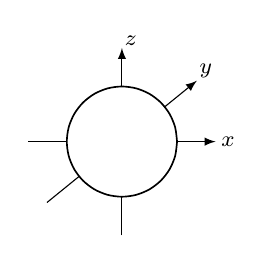
\begin{tikzpicture}[scale=0.7,z={(0.8,0.65)}]
                    \footnotesize
                    \draw [-latex] (-1.7,0,0) -- (1.7,0,0) node[right=-1pt]{$x$};
                    \draw [-latex] (0,0,-1.7) -- (0,0,1.7) node[above right=-2pt]{$y$};
                    \draw [-latex] (0,-1.7,0) -- (0,1.7,0) node[above right=-2pt]{$z$};
                    \filldraw [semithick,fill=white] plot[domain=0:2*pi,smooth,variable=\thta] ({\thta r}:1);
                \end{tikzpicture}
                \caption{$s$ orbital.}
                \label{fig:orbitals-spda}
            \end{subfigure}\\[1em]
            \begin{subfigure}[b]{0.19\linewidth}
                \centering
                \begin{tikzpicture}[scale=0.7,z={(0.8,0.65)}]
                    \footnotesize
                    \draw [-latex] (-1.7,0,0) -- (1.7,0,0) node[right=-1pt]{$x$};
                    \draw [-latex] (0,-1.7,0) -- (0,1.7,0) node[above right=-2pt]{$z$};
                    \filldraw [semithick,fill=orz] ({-6^0.5/4},0,0) circle (6^0.5/4);
                    \draw [-latex] (0,0,-1.7) -- (0,0,1.7) node[above right=-2pt]{$y$};
                    \filldraw [semithick,fill=white] ({6^0.5/4},0,0) circle (6^0.5/4);
                \end{tikzpicture}
                \caption{$p_x$ orbital.}
                \label{fig:orbitals-spdb}
            \end{subfigure}
            \begin{subfigure}[b]{0.19\linewidth}
                \centering
                \begin{tikzpicture}[scale=0.7,z={(0.8,0.65)}]
                    \footnotesize
                    \filldraw [semithick,fill=white] (0,0,{6^0.5/4}) circle (6^0.5/4);
                    \draw [-latex] (-1.7,0,0) -- (1.7,0,0) node[right=-1pt]{$x$};
                    \draw [-latex] (0,-1.7,0) -- (0,1.7,0) node[above right=-2pt]{$z$};
                    \filldraw [semithick,fill=orz] (0,0,{-6^0.5/4}) circle (6^0.5/4);
                    \draw [-latex] (0,0,-1.7) -- (0,0,-0.85) (0,0,{6^0.5/2}) -- (0,0,1.7) node[above right=-2pt]{$y$};
                \end{tikzpicture}
                \caption{$p_y$ orbital.}
                \label{fig:orbitals-spdc}
            \end{subfigure}
            \begin{subfigure}[b]{0.19\linewidth}
                \centering
                \begin{tikzpicture}[scale=0.7,z={(0.8,0.65)}]
                    \footnotesize
                    \draw [-latex] (-1.7,0,0) -- (1.7,0,0) node[right=-1pt]{$x$};
                    \draw [-latex] (0,-1.7,0) -- (0,1.7,0) node[above right=-2pt]{$z$};
                    \filldraw [semithick,fill=orz] (0,{-6^0.5/4},0) circle (6^0.5/4);
                    \draw [-latex] (0,0,-1.7) -- (0,0,1.7) node[above right=-2pt]{$y$};
                    \filldraw [semithick,fill=white] (0,{6^0.5/4},0) circle (6^0.5/4);
                \end{tikzpicture}
                \caption{$p_z$ orbital.}
                \label{fig:orbitals-spdd}
            \end{subfigure}\\[1em]
            \begin{subfigure}[b]{0.19\linewidth}
                \centering
                \begin{tikzpicture}[scale=0.7,z={(0.8,0.65)}]
                    \footnotesize
                    \draw [-latex] (-1.7,0,0) -- (1.7,0,0) node[right=-1pt]{$x$};
                    \draw [-latex] (0,-1.7,0) -- (0,1.7,0) node[above right=-2pt]{$z$};
                    \filldraw [semithick,fill=white] plot [domain=0.63:2.51,smooth,variable=\thta] ({\thta r}:{0.5*2.5^0.5*(3*sin(\thta r)^2-1)});
                    \filldraw [semithick,fill=white] plot [domain=3.75:5.67,smooth,variable=\thta] ({\thta r}:{0.5*2.5^0.5*(3*sin(\thta r)^2-1)});
                    \draw [-latex] (0,0,-1.7) -- (0,0,1.7) node[above right=-2pt]{$y$};
                    \filldraw [semithick,fill=orz] (-0.4,0,0) arc[start angle=120,end angle=60,x radius=0.8cm,y radius=0.9cm] arc[start angle=-60,end angle=-120,x radius=0.8cm,y radius=0.9cm];
                    \filldraw [semithick,fill=white] ({0.73 r}:{0.5*2.5^0.5*(3*sin(0.73 r)^2-1)}) to[out=-125,in=-55] ({2.41 r}:{0.5*2.5^0.5*(3*sin(2.41 r)^2-1)});
                \end{tikzpicture}
                \caption{$d_{z^2}$ orbital.}
                \label{fig:orbitals-spde}
            \end{subfigure}
            \begin{subfigure}[b]{0.19\linewidth}
                \centering
                \begin{tikzpicture}[scale=0.7,z={(0.8,0.65)}]
                    \footnotesize
                    \draw [-latex] (-1.7,0,0) -- (1.7,0,0) node[right=-1pt]{$x$};
                    \draw [-latex] (0,-1.7,0) -- (0,1.7,0) node[above right=-2pt]{$z$};
                    \filldraw [semithick,fill=white,scale=1.5] plot [domain=-pi:-pi/2,smooth,variable=\thta] ({\thta r}:{15^0.5/2*cos(\thta r)*sin(\thta r)});
                    \filldraw [semithick,fill=orz,scale=1.5] plot [domain=-pi/2:0,smooth,variable=\thta] ({\thta r}:{15^0.5/2*cos(\thta r)*sin(\thta r)});
                    \draw [-latex] (0,0,-1.7) -- (0,0,1.7) node[above right=-2pt]{$y$};
                    \filldraw [semithick,fill=white,scale=1.5] plot [domain=0:pi/2,smooth,variable=\thta] ({\thta r}:{15^0.5/2*cos(\thta r)*sin(\thta r)});
                    \filldraw [semithick,fill=orz,scale=1.5] plot [domain=pi/2:pi,smooth,variable=\thta] ({\thta r}:{15^0.5/2*cos(\thta r)*sin(\thta r)});
                \end{tikzpicture}
                \caption{$d_{xz}$ orbital.}
                \label{fig:orbitals-spdf}
            \end{subfigure}
            \begin{subfigure}[b]{0.19\linewidth}
                \centering
                \begin{tikzpicture}[scale=0.7,z={(0.8,0.65)}]
                    \footnotesize
                    \filldraw [semithick,fill=orz,rotate=25,xscale=1.2,yscale=1.3] plot [domain=pi/2:pi,smooth,variable=\thta] ({\thta r}:{15^0.5/2*cos(\thta r)*sin(\thta r)});
                    \filldraw [semithick,fill=white,rotate=25,scale=1.5] plot [domain=0:pi/2,smooth,variable=\thta] ({\thta r}:{15^0.5/2*cos(\thta r)*sin(\thta r)});
                    \draw [-latex] (-1.7,0,0) -- (1.7,0,0) node[right=-1pt]{$x$};
                    \draw [-latex] (0,-1.7,0) -- (0,1.7,0) node[above right=-2pt]{$z$};
                    \filldraw [semithick,fill=white,rotate=25,scale=1.5] plot [domain=-pi:-pi/2,smooth,variable=\thta] ({\thta r}:{15^0.5/2*cos(\thta r)*sin(\thta r)});
                    \draw [-latex] (0,0,-1.7) -- (0,0,1.7) node[above right=-2pt]{$y$};
                    \filldraw [semithick,fill=orz,rotate=25,xscale=1.2,yscale=1.3] plot [domain=-pi/2:0,smooth,variable=\thta] ({\thta r}:{15^0.5/2*cos(\thta r)*sin(\thta r)});
                \end{tikzpicture}
                \caption{$d_{yz}$ orbital.}
                \label{fig:orbitals-spdg}
            \end{subfigure}
            \begin{subfigure}[b]{0.19\linewidth}
                \centering
                \begin{tikzpicture}[scale=0.7,z={(0.8,0.65)}]
                    \footnotesize
                    \filldraw [semithick,fill=orz,scale=1.3,rotate=40] plot [domain=-pi/2:pi/2,smooth,variable=\thta] ({\thta r}:{15^0.5/4*cos(\thta r)^2});
                    \draw [-latex] (-1.7,0,0) -- (1.7,0,0) node[right=-1pt]{$x$};
                    \draw [-latex] (0,-1.7,0) -- (0,1.7,0) node[above right=-2pt]{$z$};
                    \filldraw [semithick,fill=white,scale=1.5] plot [domain=pi/2:3*pi/2,smooth,variable=\thta] ({\thta r}:{15^0.5/4*cos(\thta r)^2});
                    \filldraw [semithick,fill=white,scale=1.5] plot [domain=-pi/2:pi/2,smooth,variable=\thta] ({\thta r}:{15^0.5/4*cos(\thta r)^2});
                    \filldraw [semithick,fill=orz,scale=1.3,rotate=40] plot [domain=pi/2:3*pi/2,smooth,variable=\thta] ({\thta r}:{15^0.5/4*cos(\thta r)^2});
                    \draw [-latex] (0,0,-1.7) -- (0,0,-1) (0,0,1.2) -- (0,0,1.7) node[above right=-2pt]{$y$};
                \end{tikzpicture}
                \caption{$d_{x^2-y^2}$ orbital.}
                \label{fig:orbitals-spdh}
            \end{subfigure}
            \begin{subfigure}[b]{0.19\linewidth}
                \centering
                \begin{tikzpicture}[scale=0.7,z={(0.8,0.65)}]
                    \footnotesize
                    \filldraw [semithick,fill=orz,scale=1.2,rotate=-60] plot [domain=pi/2:3*pi/2,smooth,variable=\thta] ({\thta r}:{15^0.5/4*cos(\thta r)^2});
                    \draw [-latex] (-1.7,0,0) -- (1.7,0,0) node[right=-1pt]{$x$};
                    \draw [-latex] (0,-1.7,0) -- (0,1.7,0) node[above right=-2pt]{$z$};
                    \filldraw [semithick,fill=white,scale=1.5,rotate=20] plot [domain=pi/2:3*pi/2,smooth,variable=\thta] ({\thta r}:{15^0.5/4*cos(\thta r)^2});
                    \draw [-latex] (0,0,-1.7) -- (0,0,1.7) node[above right=-2pt]{$y$};
                    \filldraw [semithick,fill=white,scale=1.5,rotate=20] plot [domain=-pi/2:pi/2,smooth,variable=\thta] ({\thta r}:{15^0.5/4*cos(\thta r)^2});
                    \filldraw [semithick,fill=orz,scale=1.4,rotate=-60] plot [domain=-pi/2:pi/2,smooth,variable=\thta] ({\thta r}:{15^0.5/4*cos(\thta r)^2});
                \end{tikzpicture}
                \caption{$d_{xy}$ orbital.}
                \label{fig:orbitals-spdi}
            \end{subfigure}
            \caption{$s$, $p$, and $d$ orbitals.}
            \label{fig:orbitals-spd}
        \end{figure}
        In Figure \ref{fig:orbitals-spd}, white shading means positive phase and orange means negative phase.\par
        Here are irreducible representations for each orbital:
        \begin{align*}
            \Gamma_s &= (1,1,1,1) = A_g\\
            \Gamma_{p_x} &= (1,-1,-1,1) = B_u\\
            \Gamma_{p_y} &= (1,-1,-1,1) = B_u\\
            \Gamma_{p_z} &= (1,1,-1,-1) = A_u\\
            \Gamma_{d_{z^2}} &= (1,1,1,1) = A_g\\
            \Gamma_{d_{xz}} &= (1,-1,1,-1) = B_g\\
            \Gamma_{d_{yz}} &= (1,-1,1,-1) = B_g\\
            \Gamma_{d_{x^2-y^2}} &= (1,1,1,1) = A_g\\
            \Gamma_{d_{xy}} &= (1,1,1,1) = A_g
        \end{align*}
    \end{proof}
    \newpage
    \item The molecule \ce{Co(CO)4(SiMe3)} has a structure based on a trigonal bipyramid. The infrared spectrum of \ce{Co(CO)4(SiMe3)} exhibits three $\nu(\ce{CO})$ stretching vibrations at 2100, 2041, and $\SI{2009}{\per\centi\meter}$. Draw the two possible structures based on the TBP geometry, assign their proper point groups, and use the infrared data to determine which is the correct structure.
    \begin{proof}[Answer]
        \begin{figure}[h!]
            \centering
            \begin{subfigure}[b]{0.35\linewidth}
                \centering
                \footnotesize
                \chemfig{Co(-[:105]OC)(-Si(<[::-60]CH_3)(>:[::-20]CH_3)(-[::60]CH_3))(-[:-105]OC)(>:[:160]OC)(<[:-150]OC)}
                \caption{Equatorial trimethylsilyl group.}
                \label{fig:structure-CoCO4SiMe3a}
            \end{subfigure}
            \begin{subfigure}[b]{0.35\linewidth}
                \centering
                \footnotesize
                \chemfig{Co(-[:-16]CO)(-[2]Si(<[::-60]CH_3)(>:[::-20]CH_3)(-[::60]H_3C))(-[6]CO)(>:[:-170]OC)(<[:-135]OC)}
                \caption{Axial trimethylsilyl group.}
                \label{fig:structure-CoCO4SiMe3b}
            \end{subfigure}
            \caption{Structures of \ce{Co(CO)4(SiMe3)}.}
            \label{fig:structure-CoCO4SiMe3}
        \end{figure}
        Note that for the sake of point group assignments, the \ce{CO} ligands will be treated as identical spheres. Additionally, the \ce{SiMe3} ligand will be treated as a sphere distinguishable from the \ce{CO} "spheres."\par\medskip 
        The structure in Figure \ref{fig:structure-CoCO4SiMe3a}: Not high or low symmetry. Has a $C_2$ axis. No perpendicular $C_2$ axes. No $\sigma_h$. Has two perpendicular $\sigma_v$ planes. Therefore, it is of the $C_{2v}$ point group.\par
        We can determine that $\Gamma_\nu=(4,0,2,2)=2A_1+B_1+B_2$ by counting how many $\overrightarrow{\ce{Co-CO}}$ vectors stay the same under each symmetry operation and decomposing by inspection. With four stretching modes that are all IR active, we can expect there to be four peaks in the infrared spectrum of \ce{Co(CO)4(SiMe3)}. Therefore, this is not the correct structure.\par\medskip
        The structure in Figure \ref{fig:structure-CoCO4SiMe3b}: Not high or low symmetry. Has a $C_3$ axis. No perpendicular $C_2$ axes. No $\sigma_h$. Has three $\sigma_v$ planes all offset by $\ang{60}$. Therefore, it is of the $C_{3v}$ point group.\par
        We can determine that $\Gamma_\nu=(4,1,2)=2A_1+E$ by counting how many $\overrightarrow{\ce{Co-CO}}$ vectors stay the same under each symmetry operation and decomposing by inspection. With four $\nu(\ce{CO})$ stretching modes that are all IR active (but two of the four being degenerate), we can expect there to be three peaks in the infrared spectrum of \ce{Co(CO)4(SiMe3)}. This confirms that this is the correct structure.
    \end{proof}
    \newpage
    \item Determine the number and symmetry types of normal vibrations in the following molecules:
    \begin{enumerate}[label={\alph*)}]
        \item \ce{H3PBH3}: with a staggered ethane-like geometry.
        \begin{proof}[Answer]
            \ce{H3PBH3} has $3(8)-6=18$ normal vibrations.\par
            Not high or low symmetry. Has a $C_3$ axis. No perpendicular $C_2$ axes. No $\sigma_h$. Has three $\sigma_v$ planes all offset by $\ang{60}$. Therefore, \ce{H3PBH3} is of the $C_{3v}$ point group.\par
            We can determine that $\Gamma_{x,y,z}=(3,0,1)$. We can also figure out that the number of atoms unmoved after applying each symmetry operation is $(8,2,4)$. Thus, $\Gamma_{3N}=(24,0,4)$. We can reduce this by inspection to $\Gamma_{3N}=6A_1+2A_2+8E$.\par
            Since $\Gamma_\text{trans}=A_1+E$ and $\Gamma_\text{rot}=A_2+E$, we have by subtraction that $\Gamma_\text{vibs}=5A_1+A_2+6E$. Thus, of the 18 normal vibrations, 5 have symmetry $A_1$, 1 has symmetry $A_2$, and 12 have symmetry $E$ (note that these 12 modes pair up into 6 pairs of vibration modes of the same type).
        \end{proof}
        \item \ce{Zr2F13^5-}: Each \ce{Zr} is seven coordinate with monocapped trigonal prismatic geometry. The cap is a bridging \ce{F} (linear \ce{Zr-F-Zr} linkage) on the unique square face of the prism. The anionic complex has an eclipsed geometry about the bridging \ce{F}.
        \begin{proof}[Answer]
            \ce{Zr2F13^5-} has $3(15)-6=39$ normal vibrations.\par
            Not high or low symmetry. Has a $C_2$ axis. Has 2 perpendicular $C_2$ axes. Has a $\sigma_h$ plane. Therefore, \ce{Zr2F13^5-} is of the $D_{2h}$ point group.\par
            We can determine that $\Gamma_{x,y,z}=(3,-1,-1,-1,-3,1,1,1)$. We can also figure out that the number of atoms unmoved after applying each symmetry operation is $(15,3,1,1,1,1,7,3)$. Thus, $\Gamma_{3N}=(45,-3,-1,-1,-3,1,7,3)$. We can reduce this as follows.
            \begin{align*}
                \hspace{-4em}a_{A_g}    &= \frac{1}{8}\sum_{R_c}g_c\chi_{\Gamma_{3N}}(R_c)\chi_{A_g}(R_c)\\
                \hspace{-4em}&= \frac{1}{8}[(1)(45)(1)+(1)(-3)(1)+(1)(-1)(1)+(1)(-1)(1)+(1)(-3)(1)+(1)(1)(1)+(1)(7)(1)+(1)(3)(1)]\\
                \hspace{-4em}&= 6
            \end{align*}
            \begin{align*}
                \hspace{-4em}a_{B_{1g}} &= \frac{1}{8}\sum_{R_c}g_c\chi_{\Gamma_{3N}}(R_c)\chi_{B_{1g}}(R_c)\\
                \hspace{-4em}&= \frac{1}{8}[(1)(45)(1)+(1)(-3)(1)+(1)(-1)(-1)+(1)(-1)(-1)+(1)(-3)(1)+(1)(1)(1)+(1)(7)(-1)+(1)(3)(-1)]\\
                \hspace{-4em}&= 4
            \end{align*}
            \begin{align*}
                \hspace{-4em}a_{B_{2g}} &= \frac{1}{8}\sum_{R_c}g_c\chi_{\Gamma_{3N}}(R_c)\chi_{B_{2g}}(R_c)\\
                \hspace{-4em}&= \frac{1}{8}[(1)(45)(1)+(1)(-3)(-1)+(1)(-1)(1)+(1)(-1)(-1)+(1)(-3)(1)+(1)(1)(-1)+(1)(7)(1)+(1)(3)(-1)]\\
                \hspace{-4em}&= 6
            \end{align*}
            \begin{align*}
                \hspace{-4em}a_{B_{3g}} &= \frac{1}{8}\sum_{R_c}g_c\chi_{\Gamma_{3N}}(R_c)\chi_{B_{3g}}(R_c)\\
                \hspace{-4em}&= \frac{1}{8}[(1)(45)(1)+(1)(-3)(-1)+(1)(-1)(-1)+(1)(-1)(1)+(1)(-3)(1)+(1)(1)(-1)+(1)(7)(-1)+(1)(3)(1)]\\
                \hspace{-4em}&= 5
            \end{align*}
            \begin{align*}
                \hspace{-4em}a_{A_u}    &= \frac{1}{8}\sum_{R_c}g_c\chi_{\Gamma_{3N}}(R_c)\chi_{A_u}(R_c)\\
                \hspace{-4em}&= \frac{1}{8}[(1)(45)(1)+(1)(-3)(1)+(1)(-1)(1)+(1)(-1)(1)+(1)(-3)(-1)+(1)(1)(-1)+(1)(7)(-1)+(1)(3)(-1)]\\
                \hspace{-4em}&= 4
            \end{align*}
            \begin{align*}
                \hspace{-4em}a_{B_{1u}} &= \frac{1}{8}\sum_{R_c}g_c\chi_{\Gamma_{3N}}(R_c)\chi_{B_{1u}}(R_c)\\
                \hspace{-4em}&= \frac{1}{8}[(1)(45)(1)+(1)(-3)(1)+(1)(-1)(-1)+(1)(-1)(-1)+(1)(-3)(-1)+(1)(1)(-1)+(1)(7)(1)+(1)(3)(1)]\\
                \hspace{-4em}&= 7
            \end{align*}
            \begin{align*}
                \hspace{-4em}a_{B_{2u}} &= \frac{1}{8}\sum_{R_c}g_c\chi_{\Gamma_{3N}}(R_c)\chi_{B_{2u}}(R_c)\\
                \hspace{-4em}&= \frac{1}{8}[(1)(45)(1)+(1)(-3)(-1)+(1)(-1)(1)+(1)(-1)(-1)+(1)(-3)(-1)+(1)(1)(1)+(1)(7)(-1)+(1)(3)(1)]\\
                \hspace{-4em}&= 6
            \end{align*}
            \begin{align*}
                \hspace{-4em}a_{B_{3u}} &= \frac{1}{8}\sum_{R_c}g_c\chi_{\Gamma_{3N}}(R_c)\chi_{B_{3u}}(R_c)\\
                \hspace{-4em}&= \frac{1}{8}[(1)(45)(1)+(1)(-3)(-1)+(1)(-1)(-1)+(1)(-1)(1)+(1)(-3)(-1)+(1)(1)(1)+(1)(7)(1)+(1)(3)(-1)]\\
                \hspace{-4em}&= 7
            \end{align*}
            Therefore, we know that $\Gamma_{3N}=6A_g+4B_{1g}+6B_{2g}+5B_{3g}+4A_u+7B_{1u}+6B_{2u}+7B_{3u}$. Since $\Gamma_\text{trans}=B_{1u}+B_{2u}+B_{3u}$ and $\Gamma_\text{rot}=B_{1g}+B_{2g}+B_{3g}$, we have by subtraction that $\Gamma_\text{vibs}=6A_g+3B_{1g}+5B_{2g}+4B_{3g}+4A_u+6B_{1u}+5B_{2u}+6B_{3u}$. Thus, of the 39 normal vibrations, 6 have symmetry $A_g$, 3 have symmetry $B_{1g}$, 5 have symmetry $B_{2g}$, 4 have symmetry $B_{3g}$, 4 have symmetry $A_u$, 6 have symmetry $B_{1u}$, 5 have symmetry $B_{2u}$, and 6 have symmetry $B_{3u}$.
        \end{proof}
    \end{enumerate}
    \newpage
    \item Benzene (\ce{C6H6}) is a planar molecule.
    \begin{enumerate}[label={\alph*)}]
        \item Assign the symmetry group.
        \begin{proof}[Answer]
            Not high or low symmetry. Has a $C_6$ axis. Has 6 perpendicular $C_2$ axes. Has a $\sigma_h$ plane. Therefore, \ce{C6H6} is of the $D_{6h}$ point group.
        \end{proof}
        \item Determine the number and symmetries of the \ce{C-H} stretching modes in benzene.
        \begin{proof}[Answer]
            We can determine that $\Gamma_\nu=(6,0,0,0,2,0,0,0,0,6,0,2)$ by counting how many $\overrightarrow{\ce{C-H}}$ vectors stay the same under each symmetry operation. We can reduce this as follows.
            \begin{align*}
                a_{A_{1g}} ={}& \frac{1}{24}\sum_{R_c}g_c\chi_{\Gamma_\nu}(R_c)\chi_{A_{1g}}(R_c)\\
                \begin{split}
                    ={}& \frac{1}{24}[(1)(6)(1)+(2)(0)(1)+(2)(0)(1)+(1)(0)(1)+(3)(2)(1)+(3)(0)(1)\\
                    & +(1)(0)(1)+(2)(0)(1)+(2)(0)(1)+(1)(6)(1)+(3)(0)(1)+(3)(2)(1)]
                \end{split}\\
                ={}& 1
            \end{align*}
            \begin{align*}
                a_{A_{2g}} ={}& \frac{1}{24}\sum_{R_c}g_c\chi_{\Gamma_\nu}(R_c)\chi_{A_{2g}}(R_c)\\
                \begin{split}
                    ={}& \frac{1}{24}[(1)(6)(1)+(2)(0)(1)+(2)(0)(1)+(1)(0)(1)+(3)(2)(-1)+(3)(0)(-1)\\
                    & +(1)(0)(1)+(2)(0)(1)+(2)(0)(1)+(1)(6)(1)+(3)(0)(-1)+(3)(2)(-1)]
                \end{split}\\
                ={}& 0
            \end{align*}
            \begin{align*}
                a_{B_{1g}} ={}& \frac{1}{24}\sum_{R_c}g_c\chi_{\Gamma_\nu}(R_c)\chi_{B_{1g}}(R_c)\\
                \begin{split}
                    ={}& \frac{1}{24}[(1)(6)(1)+(2)(0)(-1)+(2)(0)(1)+(1)(0)(-1)+(3)(2)(1)+(3)(0)(-1)\\
                    & +(1)(0)(1)+(2)(0)(-1)+(2)(0)(1)+(1)(6)(-1)+(3)(0)(1)+(3)(2)(-1)]
                \end{split}\\
                ={}& 0
            \end{align*}
            \begin{align*}
                a_{B_{2g}} ={}& \frac{1}{24}\sum_{R_c}g_c\chi_{\Gamma_\nu}(R_c)\chi_{B_{2g}}(R_c)\\
                \begin{split}
                    ={}& \frac{1}{24}[(1)(6)(1)+(2)(0)(-1)+(2)(0)(1)+(1)(0)(-1)+(3)(2)(-1)+(3)(0)(1)\\
                    & +(1)(0)(1)+(2)(0)(-1)+(2)(0)(1)+(1)(6)(-1)+(3)(0)(-1)+(3)(2)(1)]
                \end{split}\\
                ={}& 0
            \end{align*}
            \begin{align*}
                a_{E_{1g}} ={}& \frac{1}{24}\sum_{R_c}g_c\chi_{\Gamma_\nu}(R_c)\chi_{E_{1g}}(R_c)\\
                \begin{split}
                    ={}& \frac{1}{24}[(1)(6)(2)+(2)(0)(1)+(2)(0)(-1)+(1)(0)(-2)+(3)(2)(0)+(3)(0)(0)\\
                    & +(1)(0)(2)+(2)(0)(1)+(2)(0)(-1)+(1)(6)(-2)+(3)(0)(0)+(3)(2)(0)]
                \end{split}\\
                ={}& 0
            \end{align*}
            \begin{align*}
                a_{E_{2g}} ={}& \frac{1}{24}\sum_{R_c}g_c\chi_{\Gamma_\nu}(R_c)\chi_{E_{2g}}(R_c)\\
                \begin{split}
                    ={}& \frac{1}{24}[(1)(6)(2)+(2)(0)(-1)+(2)(0)(-1)+(1)(0)(2)+(3)(2)(0)+(3)(0)(0)\\
                    & +(1)(0)(2)+(2)(0)(-1)+(2)(0)(-1)+(1)(6)(2)+(3)(0)(0)+(3)(2)(0)]
                \end{split}\\
                ={}& 1
            \end{align*}
            \begin{align*}
                a_{A_{1u}} ={}& \frac{1}{24}\sum_{R_c}g_c\chi_{\Gamma_\nu}(R_c)\chi_{A_{1u}}(R_c)\\
                \begin{split}
                    ={}& \frac{1}{24}[(1)(6)(1)+(2)(0)(1)+(2)(0)(1)+(1)(0)(1)+(3)(2)(1)+(3)(0)(1)\\
                    & +(1)(0)(-1)+(2)(0)(-1)+(2)(0)(-1)+(1)(6)(-1)+(3)(0)(-1)+(3)(2)(-1)]
                \end{split}\\
                ={}& 0
            \end{align*}
            \begin{align*}
                a_{A_{2u}} ={}& \frac{1}{24}\sum_{R_c}g_c\chi_{\Gamma_\nu}(R_c)\chi_{A_{2u}}(R_c)\\
                \begin{split}
                    ={}& \frac{1}{24}[(1)(6)(1)+(2)(0)(1)+(2)(0)(1)+(1)(0)(1)+(3)(2)(-1)+(3)(0)(-1)\\
                    & +(1)(0)(-1)+(2)(0)(-1)+(2)(0)(-1)+(1)(6)(-1)+(3)(0)(1)+(3)(2)(1)]
                \end{split}\\
                ={}& 0
            \end{align*}
            \begin{align*}
                a_{B_{1u}} ={}& \frac{1}{24}\sum_{R_c}g_c\chi_{\Gamma_\nu}(R_c)\chi_{B_{1u}}(R_c)\\
                \begin{split}
                    ={}& \frac{1}{24}[(1)(6)(1)+(2)(0)(-1)+(2)(0)(1)+(1)(0)(-1)+(3)(2)(1)+(3)(0)(-1)\\
                    & +(1)(0)(-1)+(2)(0)(1)+(2)(0)(-1)+(1)(6)(1)+(3)(0)(-1)+(3)(2)(1)]
                \end{split}\\
                ={}& 1
            \end{align*}
            \begin{align*}
                a_{B_{2u}} ={}& \frac{1}{24}\sum_{R_c}g_c\chi_{\Gamma_\nu}(R_c)\chi_{B_{2u}}(R_c)\\
                \begin{split}
                    ={}& \frac{1}{24}[(1)(6)(1)+(2)(0)(-1)+(2)(0)(1)+(1)(0)(-1)+(3)(2)(-1)+(3)(0)(1)\\
                    & +(1)(0)(-1)+(2)(0)(1)+(2)(0)(-1)+(1)(6)(1)+(3)(0)(1)+(3)(2)(-1)]
                \end{split}\\
                ={}& 0
            \end{align*}
            \begin{align*}
                a_{E_{1u}} ={}& \frac{1}{24}\sum_{R_c}g_c\chi_{\Gamma_\nu}(R_c)\chi_{E_{1u}}(R_c)\\
                \begin{split}
                    ={}& \frac{1}{24}[(1)(6)(2)+(2)(0)(1)+(2)(0)(-1)+(1)(0)(-2)+(3)(2)(0)+(3)(0)(0)\\
                    & +(1)(0)(-2)+(2)(0)(-1)+(2)(0)(1)+(1)(6)(2)+(3)(0)(0)+(3)(2)(0)]
                \end{split}\\
                ={}& 1
            \end{align*}
            \begin{align*}
                a_{E_{2u}} ={}& \frac{1}{24}\sum_{R_c}g_c\chi_{\Gamma_\nu}(R_c)\chi_{E_{2u}}(R_c)\\
                \begin{split}
                    ={}& \frac{1}{24}[(1)(6)(2)+(2)(0)(-1)+(2)(0)(-1)+(1)(0)(2)+(3)(2)(0)+(3)(0)(0)\\
                    & +(1)(0)(-2)+(2)(0)(1)+(2)(0)(1)+(1)(6)(-2)+(3)(0)(0)+(3)(2)(0)]
                \end{split}\\
                ={}& 0
            \end{align*}
            Therefore, we know that $\Gamma_\nu=A_{1g}+E_{2g}+B_{1u}+E_{1u}$. Thus, there are 6 \ce{C-H} stretching modes in benzene: 1 with symmetry $A_{1g}$, 2 with symmetry $E_{2g}$ (note that these 2 modes form a pair vibration modes of the same type), 1 with symmetry $B_{1u}$, and 2 with symmetry $E_{1u}$ (again, these pair up).
        \end{proof}
        \item Determine the Raman and infrared activities for each vibration.
        \begin{proof}[Answer]
            Since the $A_{1g}$, $E_{1g}$, and $E_{2g}$ irreducible representations are Raman active, we know that the $A_{1g}$ and $E_{2g}$ \ce{C-H} stretching modes are Raman active. The others are Raman silent. Additionally, since the $A_{2u}$ and $E_{1u}$ irreducible representations are IR active and two of the \ce{C-H} stretching vibration modes are of the $E_{1u}$ type, the $E_{1u}$ vibrations are both IR active. The others are IR silent.
        \end{proof}
    \end{enumerate}
\end{enumerate}




\end{document}